\documentclass[a4paper,12pt]{report}

\usepackage[italian]{babel}
\usepackage{hyperref}
\usepackage[utf8]{inputenc}
\usepackage{float}
\usepackage{xcolor}
\usepackage{graphicx}

\title{\textbf{CineRadar}\\Progetto di Basi di dati}
\author{Martin Tomassi; 0001077737\\Francesco Pazzaglia; 0001077423\\Luca Casadei; 0001069237}
\date{\today}

\begin{document}
	\maketitle
	\tableofcontents
	\chapter{Analisi dei requisiti}
	\section{Introduzione}
	Il progetto consiste nella realizzazione di un applicativo per la condivisione e la recensione di elementi multimediali quali film e serie TV.
	\section{Intervista}
	È richiesto un sistema che consenta all'utenza di accedere al portale di condivisione di film e serie TV e poter recensirne uno o più di interesse, \textit{(D'ora in poi entrambi li denomineremo "film" in maniera generica)}. È necessario che l'utente si registri inserendo i propri dati che verranno salvaguardati, tra cui username, password, nome, cognome, data di nascita per controllare i limiti di età sui film. Un utente deve avere la possibilità di aggiungere nuovi film nel sistema, ma non in maniera diretta, la richiesta deve prima essere approvata da un altro tipo di utente con privilegi di amministratore del sistema. L'amministratore si occuperà di aggiungere film alla piattaforma con frequenza settimanale. Sulle recensioni di altri utenti, un visualizzatore registrato può esprimere un parere di utilità che andrà a classificare la recensione in una sorta di "classifica delle recensioni più utili". Quando si va a memorizzare un film bisogna inserire il titolo, uno o più autori, la descrizione, la durata, l'anno di rilascio ed eventuale casa produttrice. I visualizzatori devono essere in grado di vedere tutti i film presenti in base a dei filtri sul genere, categoria, autori e recensioni, sempre a patto che i risultati ottenuti rispettino i limiti di età standard dei film (\textit{over 18, over 16} etc\dots). Quando un utente vede un film della lista, deve poterlo segnare come \textit{"già visto"} per poterlo recensire successivamente se lo desidera. Dato che si vogliono anche incentivare le famiglie, è richiesta una funzionalità che renda possibile inserire un'età e visualizzare i film la cui visione è consentita (per esempio per capire se un film è adatto per il proprio figlio). Vi devono essere anche delle piccole classifiche per incentivare gli utenti ad effettuare recensioni, per esempio una classifica degli utenti con il maggior numero di film visualizzati o recensiti. Vi è inoltre una statistica sui film inseriti, per esempio sarà possibile ottenere il genere di film con il maggior numero di visualizzazioni complessive. Oltre che sui film ci devono essere delle statistiche su chi i film li fa, quindi per esempio il regista che ha girato il film con le recensioni migliori. L'amministratore può attribuire dei premi in base alla classifica degli utenti migliori (in base alle recensioni più utili), effettuerà anche atti di moderazione sugli utenti registrati, ad esempio, se un utente effettua troppe recensioni al di sotto della soglia di utilità potrà essere rimosso dal sistema.
	\section{Estrazione dei dati dell'intervista}
	\textbf{Utente / Visualizzatore} $\longrightarrow$ Utente che si registra sull'applicativo\\Successivamente verranno elencati i dati da dover memorizzare.
	\begin{itemize}
		\item Nome
		\item Cognome
		\item Data di nascita
		\item Username
		\item Password
	\end{itemize}
	\textbf{Amministratore} $\longrightarrow$ Utente privilegiato che effettua operazioni di moderazione e inserimento dati. Dato che nell'intervista non emergono i dati da memorizzare per l'amministratore, si presuppone che vi sia un contatto per poterlo raggiungere, oltre che alle credenziali.
	\begin{itemize}
		\item Username
		\item Password
		\item Contatto (Da stabilire se uno o più)
	\end{itemize}
	\textbf{Film / Serie TV} $\longrightarrow$ Elementi multimediali su cui gli utenti registrati possono apporre la propria visualizzazione ed effettuare recensioni in seguito.
	\begin{itemize}
		\item Data di rilascio
		\item Titolo
		\item Descrizione
		\item Genere
		\item Limite di età
	\end{itemize}
	\textbf{Autori / Registi} $\longrightarrow$ Questi vengono memorizzati per stilare la classifica visualizzabile, ed esplicitare delle preferenze.
	\begin{itemize}
		\item Nome
		\item Cognome
		\item Nome d'arte
		\item Età
	\end{itemize}
	\subsection*{Termini da chiarire}
	\begin{itemize}
		\item "Visto" $\longrightarrow$ Un utente può spuntare una casella "visto" se ha visto effettivamente il film, si può recensire un film solo se è stato spuntato come "visto".
		\item "Filtro" $\longrightarrow$ Un filtro viene applicato sulla ricerca che può fare un utente sulla lista di film / serie, questo può riguardare l'autore, il titolo, le recensioni dell'utenza etc\dots
	\end{itemize}
	\subsection*{Elenco delle azioni}
	\subsubsection{Utente}
	\begin{itemize}
		\item Registrarsi sulla piattaforma.
		\item Accedere alla piattaforma.
		\item Scegliere le proprie categorie di preferenza.
		\item Visualizzare i film/serie in base ai filtri scelti e ai limiti di età.
		\item Data un età inferiore alla propria, ottenere la lista dei film che sono visualizzabili con quell'età.
		\item Richiedere all'amministratore l'aggiunta di un film / serie non presente in elenco.
		\item Contrassegnare come visualizzato un film / serie.
		\item Recensire i film contrassegnati come visualizzati.
		\item Dare una valutazione di utilità alle recensioni degli altri utenti.
		\item Ricercare dei film in base al genere o all'autore.
		\item Visualizzare le classifiche degli autori e dei generi.
	\end{itemize}
	\subsubsection{Amministratore}
	\begin{itemize}
		\item Ottenere le statistiche degli utenti registrati alla piattaforma per poter effettuare attività di moderazione, tra cui: 
		\begin{itemize}
			\item (S)Bloccare o eliminare l'accesso ad un utente alla piattaforma se ha effettuato troppe recensioni che stanno sotto alla soglia di utilità.
			\item Premiare l'utente in cima alla classifica delle recensioni più utili (il premio è una targhetta che comparirà accanto al nome).
		\end{itemize}
		\item Aggiungere film / serie alla lista, compresi quelli che sono stati richiesti dagli utenti.
		\item Inserire nuovi autori o registi da associare a dei film.
	\end{itemize}
	\chapter{Progettazione concettuale}
	\section{Schema scheletro}
	\subsection{Utenza}
	Rappresentazione di una sottoparte dello schema ER che riguarda la gestione dell'utenza, in particolare, è stata pensata una generalizzazione dell'entità \textbf{utente} con due sotto-entità \textbf{amministratore} e \textbf{visualizzatore} di cui dobbiamo memorizzare elementi diversi. La generalizzazione è di tipo \textit{totale} e \textit{esclusiva}, questo perché l'amministratore ha un tipo di account diverso da quello di semplice visualizzatore, se l'amministratore vuole effettuare le operazioni di un utente normale deve registrarsi con un altro account.
	\begin{figure}[H]
		\centering
		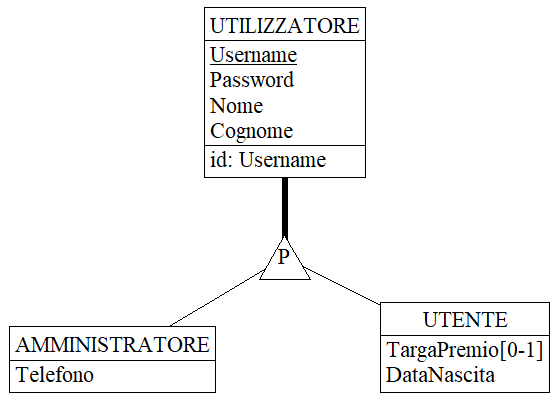
\includegraphics[width=300pt]{ER/utenza.png}
		\caption{Scheletro dello schema ER dell'utenza.}
	\end{figure}
\end{document}